\documentclass[12pt,chapterheads]{ucsd}

%% math packages
\usepackage{amsmath, amscd, amssymb, amsthm}

%% graphic packages
\usepackage{scrextend}
\usepackage{pslatex}
\usepackage{graphicx}

%% caption stuff
\makeatletter
\gdef\@ptsize{2}% 12pt documents
\let\@currsize\normalsize
\makeatother
\usepackage{setspace}
\doublespace
\usepackage[font=small, width=0.9\textwidth]{caption}

%% SUBFIG - Use this to place multiple images in a
%    single figure.  Subfig will handle placement and
%    proper captioning (e.g. Figure 1.2(a))
% \usepackage{subfig}

%% font stuff (for TImes New Roman)
\usepackage[T1]{fontenc}
\usepackage{mathptmx}

%% INDEX
%   Uncomment the following two lines to create an index: 
% \usepackage{makeidx}
% \makeindex
%   You will need to uncomment the \printindex line near the
%   bibliography to display the index.  Use the command
% \index{keyword} 
%   within the text to create an entry in the index for keyword.
%   To compile a LaTeX document with an index the 'makeindex'
%   command will need to be run.  See the wiki for more details.

%% URL stuff
\usepackage{url}
\urlstyle{same}

%% citation stuff
\usepackage{microtype}  % avoids citations that hang into the margin

%% footnote stuff
\usepackage{footnote}
\makesavenoteenv{tabular}
\makesavenoteenv{table}

%% table formatting stuff
\usepackage{rotating}  % Enables the sideways environment (NCPW)
\usepackage{array}  % Enables "m" tabular environment http://ctan.org/pkg/array
\usepackage{booktabs}  % Enables \toprule  http://ctan.org/pkg/array
\newcolumntype{P}[1]{>{\centering\arraybackslash}m{#1}}

%% acronym/abbreviation stuff
\usepackage[acronym]{glossaries}

%% define section names
\newcommand{\abbrevtitle}{List of Abbreviations}
\newcommand{\introtitle}{Introduction}
\newcommand{\favitestitle}{FAVITES: simultaneous simulation of transmission networks, phylogenetic trees, and sequences}

%% define acronyms
\newacronym{API}{API}{Application Program Interface}
\newacronym{ART}{ART}{Antiretroviral Therapy}
\newacronym{BA}{BA}{Barab\'asi--Albert}
\newacronym{ER}{ER}{Erd\H os--R\'enyi}
\newacronym{GTR}{GTR}{General Time-Reversible}
\newacronym{HIV}{HIV}{Human Immunodeficiency Virus}
\newacronym{HMM}{HMM}{Hidden Markov Model}
\newacronym{LTT}{LTT}{Lineages Through Time}
\newacronym{MSA}{MSA}{Multiple Sequence Alignment}
\newacronym{WS}{WS}{Watts--Strogatz}
\makeglossaries


\begin{document}

%% include sections
%% Dissertation Info
\title{Mathematical Modeling of Viral Evolution and Epidemiology}
\author{Alexander Niema Moshiri}
\degreeyear{2019}
\degreetitle{Doctor of Philosophy}
\field{Bioinformatics and Systems Biology}
%\specialization{Anthropogeny}  % If you have a specialization, add it here

%% Committee Info
\chair{Professor Siavash Mirarab}
\cochair{Professor Pavel A. Pevzner}
\othermembers{
Professor Vineet Bafna\\
Professor David M. Smith\\
Professor Joel O. Wertheim\\
}
\numberofmembers{5} % |chair| + |cochair| + |othermembers|

%% Define Acknowledgement Statements (to avoid typos when copying)
\newcommand{\ackfavites}{Chapter~\ref{chap:favites}, in full, is a reprint of the material as it appears in ``\favitestitle'' (2018). Moshiri, Niema; Ragonnet-Cronin, Manon; Wertheim, Joel; Mirarab, Siavash, \textit{Bioinformatics}, bty921. The dissertation author was the primary investigator and first author of this paper.}
\newcommand{\ackdualbirth}{Chapter~\ref{chap:dualbirth}, in full, is a reprint of the material as it appears in ``\dualbirthtitle'' (2017). Moshiri, Niema; Mirarab, Siavash, \textit{Systematic Biology}, 67(3), 475-489. The dissertation author was the primary investigator and first author of this paper.}
\newcommand{\ackproact}{Chapter~\ref{chap:proact}, in full, has been submitted for publication of the material as it may appear in ``\proacttitle'' (2019) Moshiri, Niema; Smith, Davey; Mirarab, Siavash, \textit{Molecular Biology and Evolution}. The dissertation author was the primary investigator and first author of this paper.}
\newcommand{\acktreeswift}{Chapter~\ref{chap:treeswift}, in full, has been submitted for publication of the material as it may appear in ``\treeswifttitle'' (2019) Moshiri, Niema, \textit{SoftwareX}. The dissertation author was the primary investigator and sole author of this paper.}

%% START FRONTMATTER
\begin{frontmatter}
\makefrontmatter

%% Dedication
\begin{dedication}
\vspace*{\fill}
I dedicate this dissertation to Ladan Moshiri, Ramin Moshiri, and Michelle Roxanna Moshiri-Warncke for years of love and support.
~\\~\\~\\
I dedicate this dissertation to Karen George for always being by my side.
~\\~\\~\\
I dedicate this dissertation to Ryan Micallef and Felix Garcia for teaching me to live my life a quarter mile at a time.
~\\~\\~\\
I dedicate this dissertation to all my friends in the Bioinformatics and Systems Biology program for some of the best memories of my life.
\vspace*{\fill}
\end{dedication}

%% Epigraph
\begin{epigraph}
\begin{center}
\begin{minipage}{0.65\linewidth}
\onehalfspacing
{\large
\textit{Folk in these stories had lots of chances of turning back, only they didn't. Because they were holding onto something.}\\
~\\
\textit{What are we holding onto, Sam?}\\
~\\
\textit{That there's some good in this world, Mr. Frodo. And it's worth fighting for.}
\begin{flushright}
---J.R.R. Tolkien
\end{flushright}
}
\end{minipage}
\end{center}
\end{epigraph}

%% Table of Contents
\tableofcontents

%% List of Abbreviations
\newpage
\addcontentsline{toc}{chapter}{\abbrevtitle}
\begin{center}\expandafter\MakeUppercase\expandafter{\abbrevtitle}\end{center}
\let\clearpage\relax
\vspace*{-2cm}
\printglossary[type=\acronymtype,title={}]

%% List of Symbols

%% List of Figures and Tables
\listoffigures
\listoftables


%% Acknowledgements
\begin{acknowledgements}
I would like to thank all of the people who have helped me throughout my Ph.D. My colleagues in the Bioinformatics and Systems Biology Graduate Program and in the Computer Science and Engineering department have been great to work with, especially Jens Luebeck, Margaret Donovan, Bill Greenwald, Ben Pullman, and Argus Athanas. I enjoyed having the support of such excellent lab mates as Erfan Sayyari, Metin Balaban, Uyen Mai, Maryam Rabiee, Sina Malekian, and Chao Zhang.
I would also like to thank Prof.~Joel Wertheim, Manon Ragonnet-Cronin, Prof.~Davey Smith, and Prof.~Sanjay Mehta for teaching so much about the molecular biology and epidemiology of HIV.
I am truly blessed to have been able to work with such amazing people.

I would not be where I am today (both figuratively and literally) without the mentorship of Prof.~Vineet Bafna. I met him early on in my undergraduate career, and he has been the source of sage wisdom throughout my entire academic career thus far. It was largely because of him that I decided to continue to pursue graduate education in Bioinformatics, and I am thankful that his guidance led me down this path.

I am grateful of Prof.~Pavel Pevzner for taking me under his wing at a time when I was somewhat lost regarding my career aspirations. Growing up, I always thought I wanted to become a medical doctor, but I always had a strong passion for technology. It was under his mentorship that I recognized the possibility to merge these two seemingly unrelated fields, and I was able to see the biomedical applications of Computer Science. He also introduced me to the field of Bioinformatics Education, and it was because of his guidance that I realized my passion for teaching, and I am honored he took a chance on me. He is truly a visionary, and I am happy to have been able to work with him.

When starting a Ph.D. program, one of the most stressful thoughts is ``Will I find a good mentor?'', and I was extremely fortunate to have found Prof.~Siavash Mirarab. I cannot thank him enough for all the time and effort he has taken to make my Ph.D. experience productive and intellectually stimulating. From the long sessions in which we'd be working on an algorithmic problem together, to the hours he would spend helping me revise my manuscripts, the effort he took to mentor me has instilled within me far more than I could have imagined. I aspire to be as brilliant of a scientist as he one day, and I hope to be as great of a mentor as he was to me.

\ackfavites

\ackdualbirth

\ackproact

\acktreeswift
\end{acknowledgements}

%% Vita
\begin{vitapage}
\begin{vita}
\item[2015] B.~S. in Bioengineering: Bioinformatics, University of California, San Diego
\item[2015-2016] Teaching Assistant, University of California, San Diego
\item[2017] Associate Instructor, University of California, San Diego
\item[2015-2019] Research Assistant, University of California, San Diego
\item[2019] Ph.~D. in Bioinformatics and Systems Biology, University of California, San Diego
\end{vita}
\begin{publications}
\item \textbf{Niema Moshiri} (2019). ``Why Do I Look Like My Mom and Dad? Plants and Animals Inherit Traits From Parents,'' \textit{STEMTaught}
\item Metin Balaban, \textbf{Niema Moshiri}, Uyen Mai, and Siavash Mirarab (2019). ``TreeCluster: Clustering Biological Sequences using Phylogenetic Trees,'' \textit{GLBIO 2019}, doi:~10.1101/591388
\item Adam Rule, Amanda Birmingham, Cristal Zuniga, Ilkay Altintas, Shih-Cheng Huang, Rob Knight, \textbf{Niema Moshiri}, Mai H. Nguyen, Sara Brin Rosenthal, Fernando Pérez, and Peter W. Rose (2019). ``Ten Simple Rules for Reproducible Research in Jupyter Notebooks,'' \textit{PLOS Computational Biology (in press)}, arXiv:~1810.08055
\item \textbf{Niema Moshiri} and Liz Izhikevich (2018). \textit{Design and Analysis of Data Structures}, Amazon KDP, ISBN:~1981017232
\item \textbf{Niema Moshiri}, Manon Ragonnet-Cronin, Joel O. Wertheim, and Siavash Mirarab (2018). ``FAVITES: simultaneous simulation of transmission networks, phylogenetic trees, and sequences,'' \textit{Bioinformatics}, doi:~10.1093/bioinformatics/bty921
%\item \textbf{Niema Moshiri} (2018). ``The dual-Barab\'asi-Albert model,'' \textit{arXiv}, arXiv:~1810.1810.10538
%\item \textbf{Niema Moshiri} (2018). ``TreeN93: a non-parametric distance-based method for inferring viral transmission clusters,'' \textit{bioRxiv}, doi:~10.1101/383190
\item \textbf{Niema Moshiri} (2018). ``TreeSwift: a massively scalable Python tree package,'' \textit{bioRxiv}, doi:~10.1101/325522
\item \textbf{Niema Moshiri}, Liz Izhikevich, and Christine Alvarado (2018). ``Data Structures: An Active Learning Approach,'' \textit{edX}
\item \textbf{Niema Moshiri}, Phillip Compeau, and Pavel Pevzner (2017). ``Analyze Your Genome!,'' \textit{edX}
\item Phillip Compeau, \textbf{Niema Moshiri}, and Pavel Pevzner (2017). ``Introduction to Genomic Data Science,'' \textit{edX}
%\item \textbf{Niema Moshiri} (2017). ``A linear-time algorithm to sample the dual-birth model,'' \textit{bioRxiv}, doi:~10.1101/226423
\item \textbf{Niema Moshiri} and Siavash Mirarab (2017). ``A Two-State Model of Tree Evolution and Its Applications to Alu Retrotransposition,'' \textit{Systematic Biology}, 67(3), 475-489. doi:~10.1093/sysbio/syx088
\end{publications}
\end{vitapage}

%% Abstract
\begin{abstract}
Phylogenetic trees can be used to study the evolution of any sequence that evolves, including viruses. In a viral epidemic, the history of transmission events defines constraints on the evolutionary history of the viral population. Models of tree evolution describe probability distributions over the space of tree shapes and can be used to simulate trees that capture the evolutionary patterns of real world phenomena as well as to infer evolutionary parameters inherently of interest to the biologist. The spread of many viruses is driven by social and sexual networks, and because of the relationship between their evolutionary and transmission histories, phylogenetic inference from viral sequences can be used to improve the inference of patterns of the epidemic, which in turn can greatly enhance epidemiological intervention. The simultaneous simulation of viral transmission network, phylogenetic tree, and sequences can provide a method to observe the effects of virus model parameters on the epidemic as well as to study the accuracies and errors of transmission inference tools. Further, the development of massively-scalable tools to analyze ultra-large datasets of viral sequences can aid epidemiologists in the real-time surveillance of the spread of disease. In an effort to contribute to these ideas, I developed a novel framework to simulate viral transmission networks, phylogenetic trees, and sequences, developed a novel evolutionary model, studied the effects of model parameters on epidemic outcomes via simulation experiments using the proposed framework, developed a scalable and non-parametric method of transmission risk prioritization, and contributed to publicly-accessible Bioinformatics education.
\end{abstract}
\end{frontmatter}

%% END FRONT MATTER
%% START INTRO CHAPTER
\addcontentsline{toc}{chapter}{\introtitle}
\chapter*{\introtitle}
\clearpage

Although they are typically associated with the study of the evolution of species, phylogenetic trees can be used to study the evolution of any sequence that evolves. For example, phylogenetic methods have been used to study the evolution of multicopy gene families~ \cite{Page1997}, cancer genomes~\cite{El-Kebir2016,Nowell1976}, antibodies~\cite{Litman1993,Robinson2015,Safonova2015}, segmental duplicates~\cite{Bailey2006,Jiang2007}, and transposable genomic elements~\cite{Dewannieux2003,Moshiri2017}, which are all entities that evolve \textit{within} the genome of a single species. Further, they can be used to study the evolution of viruses, both within and across hosts~\cite{Frost2001,Lemey2006,Vrancken2014}. In the case of viruses, the history of transmission events constrains the evolutionary history, such as imposing a bottleneck at the time of each transmission~\cite{Carlson2014}.

The spread of many infectious diseases is driven by social and sexual networks~\cite{Rivas2012}, and reconstruction of their transmission histories from molecular data can greatly enhance intervention. For example, network-based statistics for measuring \gls{HIV} treatment effects can yield increased statistical power~\cite{Wertheim2011}; the analysis of the growth of \gls{HIV} infection clusters can yield actionable epidemiological information for disease treatment and prevention~\cite{Aldous2012,Brenner2013}; transmission-aware models can be used to infer rates of \gls{HIV} evolution~\cite{Vrancken2014}. The ability to infer properties and patterns of the transmission history of a viral epidemic allows public health officials to intervene and attempt to prevent the spread of the virus. In the case of \gls{HIV}, patients who adhere to \gls{ART} can become ``virally suppressed,'' meaning the virus is kept at bay, resulting in slower progression of the \gls{HIV} disease as well as a significant reduction in transmission risk~\cite{AIDSinfo2019}. Thus, the ability to predict which individuals are most at-risk of transmitting the virus would provide public health officials actionable information: they can take measures to ensure high-risk individuals are able to continuously adhere to \gls{ART}.

The ability to infer and reconstruct properties of a transmission network has been researched extensively in recent years~\cite{Wertheim2017,Ragonnet-Cronin2019}, and many tools exist that attempt to use molecular data to try to perform this inference~\cite{Rose2017}. For example, PhyloPart~\cite{Prosperi2011}, Cluster Picker~\cite{Ragonnet-Cronin2013}, and TreeCluster~\cite{Balaban2019} infer transmission clusters using phylogenies inferred from viral sequences. HIV-TRACE, on the other hand, infers transmission clusters directly from sequences~\cite{Pond2018}. While these tools have been used to analyze real datasets~\cite{Campbell2017}, the accuracies, errors, and limitations of these methods are still poorly understood.

By utilizing models of social contact networks, viral transmission, tree evolution, and sequence evolution together, epidemiologists can define complex probabilistic distributions composed of sub-models. These complex distributions can be sampled to simulate data representative of a virus of interest as it spreads through a population of interest, and the resulting data can be used to evaluate the accuracies of transmission network inference methods as well as to study trends and patterns of an epidemic as a function of the various model parameters to gain insights into the mechanisms driving the epidemic of interest~\cite{Ratmann2017}. However, many existing tools to perform such epidemic simulations have model assumptions that the user cannot relax or change. In Chapter~\ref{chap:favites}, I will discuss FAVITES: a novel epidemic simulation framework I developed that provides flexibility in terms of the model assumptions about the epidemic, allowing the user to control the generative model in minute detail. The framework is defined by a series of interactions of abstract modules, and each \textit{implementation} of a module defines the model assumptions. Thus, users are free to select whichever module implementations (and thus model assumptions) that best fit their epidemic of interest. In addition to presenting the tool, I will describe in detail a simulation experiment designed to emulate the San Diego \gls{HIV} epidemic between 2005 and 2014, and I will use the simulated data to compare and contrast existing transmission clustering methods.

Of course, the ability to simulate an epidemic depends entirely on the existence of statistical models that appropriately describe the processes of the epidemic of interest. Models of tree evolution describe probability distributions over the space of tree shapes~\cite{Yule1925,Aldous2001}, which can be used as the prior distribution in a Bayesian inference~\cite{Drummond2007,Mooers2012,Sayyari2016}, to generate null distributions describing certain neutral processes~\cite{Guyer1991,Kirkpatrick1993,Agapow2002}, or to infer evolutionary parameters inherently of interest to the biologist~\cite{Morlon2014}. Similarly, generalized epidemic models describe probability distributions over the space of transmission networks~\cite{Sahneh2013}, and simulations that sample the distributions defined by these stochastic models allows epidemiologists to study infection patterns of disease epidemics~\cite{Sahneh2017}. Further, network models describe probability distributions over graphs, and they can be used to capture features of networks of interactions (e.g. social interactions between humans)~\cite{Watts1998,Watts1999,Barabasi1999,Erdos1959}. Lastly, models of sequence evolution describe the mutation of a sequence over time~\cite{Jukes1969,Kimura1980,Felsenstein1981,Tamura1993,Tavare1986}, and they can be used to simulate the evolution of a sequence down a phylogeny~\cite{Rambaut1997} as well as to infer the evolutionary history of a set of sequences~\cite{Felsenstein2003}. In the case of retroviruses and retrotransposons, which replicate via reverse transcription~\cite{Whitcomb1992} and may undergo significant selection pressure~\cite{Wood2009}, a neutral model of tree evolution like the Yule~\cite{Yule1925} or Coalescent~\cite{Kingman1982} may not be appropriate. In Chapter~\ref{chap:dualbirth}, I will discuss the dual-birth model, a novel model of tree evolution that is motivated by the retrotransposition of \textit{Alu} elements in the human genome~\cite{Batzer2002}. I will derive various probabilistic distributions and theoretical expectations of trees sampled under the model, and I will then present two approaches for estimating model parameters from a given phylogeny. I will then present the results of an analysis of close to one million \textit{Alu} sequences from the human genome in which I infer the dual-birth model parameters and present an estimate of the number of active \textit{Alu} elements, a topic of much debate~\cite{Price2004,Deininger2011,Cordaux2004}.

The goal of many transmission clustering analyses is to learn about the dynamics of a virus through a given population, often to try to predict which sub-populations may be spreading the virus more rapidly~\cite{Wertheim2011,Wertheim2017,Little2014}. However, transmission clustering is essentially a way of summarizing the relationships between the sampled viral sequences, and instead of performing predictions and inferences on these summaries, what if we were able to infer properties of interest directly from the evolutionary relationships of the viruses? In Chapter~\ref{chap:proact}, I investigate a single specific question: Given a set of viral sequences sampled from people living with \gls{HIV}, can I predict which individuals are most at-risk of transmitting the virus in the future? In an attempt to address this question, I present ProACT, a tool that attempts to prioritize people living with \gls{HIV} based on risk of future transmissions. ProACT depends only on the viral phylogeny and does not require any demographic information from the patients, meaning it is not sensitive to error-prone survey data, and most importantly, it is less prone to bias.

A primary focus of mine is the ability to execute phylogenetic methods like ProACT in a massively-scalable fashion. The scalability of a computational tool is primarily dependant on two things: (1) the theoretical time complexity of the algorithm, and (2) the efficiency of the implementation of the algorithm. While developing FAVITES and ProACT, I found that, although the phylogenetic algorithms I designed were quite fast in theory, my implementations using existing tree-manipulation packages were much slower than I anticipated due to significant overhead in loading and initializing my ultra-large phylogenies. In Chapter~\ref{chap:treeswift}, I will present TreeSwift, a new Python package for traversing and manipulating trees. I will describe its implementation design, demonstrate some of its features, and compare its execution time for various common tree algorithms against existing packages.

As can be seen, as the cost of sequencing decreases, the amount of viral sequence data available to researchers is growing rapidly, and as a result, the field of Epidemiology is becoming increasingly dependent on scalable computational methods. However, many researchers in the fields of Epidemiology and Molecular Biology have never received formal education in computation. In recent years, computational courses have started appearing in undergraduate Biology major curricula, and while this will provide computational skills to the next generation of biomedical and epidemiological researchers, it does not benefit the current generation of professionals. In Chapter~\ref{chap:education}, I will present my contributions to Bioinformatics education in the form of developing novel \glspl{MOOC} and \glspl{MAIT}, and I will discuss the pedagogical philosophy I employed in developing my learning materials.

In summary, I show that modern studies in viral epidemiology require the ability to perform simulation experiments that can appropriately capture the virus and population of interest, which thus requires tools to run such simulations efficiently as well as statistical models that make realistic assumptions. I also show that the ability to infer actionable epidemiological information from molecular data is an open problem. In this dissertation, I present a novel framework for epidemic simulations, provide a novel model of phylogenetic evolution (and derive probabilistic distributions and theoretical expectations of trees sampled under the model), demonstrate the effectiveness of a novel phylogenetic tool for prioritizing people living with \gls{HIV} based on their risk of future transmissions, and introduce a novel package for performing tree traversals and manipulations efficiently on ultra-large phylogenies. I also discuss my contributions to Bioinformatics education.

%% END INTRO CHAPTER
%% START FAVITES CHAPTER
\chapter{\favitestitle}
\label{chap:favites}
\newpage

\textit{Motivation} --- The ability to simulate epidemics as a function of model parameters allows insights that are unobtainable from real datasets. Further, reconstructing transmission networks for fast-evolving viruses like \gls{hiv} may have the potential to greatly enhance epidemic intervention, but transmission network reconstruction methods have been inadequately studied, largely because it is difficult to obtain ``truth'' sets on which to test them and properly measure their performance.

\textit{Results} --- We introduce FAVITES, a robust framework for simulating realistic datasets for epidemics that are caused by fast-evolving pathogens like \gls{hiv}. FAVITES creates a generative model to produce contact networks, transmission networks, phylogenetic trees, and sequence datasets, and to add error to the data. FAVITES is designed to be extensible by dividing the generative model into modules, each of which is expressed as a fixed API that can be implemented using various models. We use FAVITES to simulate \gls{hiv} datasets and study the realism of the simulated datasets. We then use the simulated data to study the impact of the increased treatment efforts on epidemiological outcomes. We also study two transmission network reconstruction methods and their effectiveness in detecting fast-growing clusters.

\textit{Availability and implementation} --- FAVITES is available at \url{https://github.com/niemasd/FAVITES}, and a Docker image  can be found on DockerHub (\url{https://hub.docker.com/r/niemasd/favites}).

\section{Introduction}
The spread of many infectious diseases is driven by social and sexual networks~\cite{Kelly1991}, and reconstructing their transmission histories from molecular data may be able to enhance intervention. For example, network-based statistics for measuring the effects of \gls{art} in \gls{hiv} can yield increased statistical power~\cite{Wertheim2011}; the analysis of the growth of HIV infection clusters can yield actionable epidemiological information for disease control~\cite{Lewis2008}; transmission-aware models can be used to infer HIV evolutionary rates~\cite{Vrancken2014}.

%% END FAVITES CHAPTER


%% Appendix
\appendix
%% START FAVITES SUPPLEMENT
\chapter{Supplemental Material for Chapter~\ref{chap:favites}}
\label{chap:favites-sup}
\clearpage

\begin{table}[!ht]
\caption[Comparison with Existing Simulation Tools]{Comparison with Existing Simulation Tools}
\vspace{-0.25in}
\begin{center}
\begin{tabular}{|P{0.8in}|P{0.5in}|P{0.8in}|P{0.8in}|P{0.6in}|P{0.8in}|P{0.8in}|}
\hline
 & \textbf{epinet} & \textbf{TreeSim} & \textbf{outbreaker} & \textbf{seedy} & \textbf{PANGEA} & \textbf{FAVITES} \\
\hline
\textbf{Contact Network} & Fixed & Complete & Complete & Complete & Fixed & Any \\
\hline
\textbf{Trans. Network} & Fixed & Fixed & Fixed & Fixed & Fixed & Any\\
\hline
\textbf{Sampling} & N/A & Fixed or \newline Sequential & Fixed & Uniform & Fixed & Any \\
\hline
\textbf{Phylogeny} & None & Fixed & Fixed & Fixed & Coalescent & Any \\
\hline
\textbf{Mutation Rate} & N/A & N/A & Constant & Constant & Fixed & Any \\
\hline
\textbf{Sequences} & None & None & Fixed & Fixed & Fixed & Any \\
\hline
\textbf{Sequencing} & N/A & N/A & No & No & No & Any \\
\hline
\end{tabular}
\end{center}
\label{tab:favites-comparison}
\end{table}

\begin{table}[!ht]
\caption[Post-Validation Tools]{Post-Validation Tools}
\vspace{-0.25in}
\begin{center}
\begin{tabular}{|P{2.3in}|P{3.7in}|}
\hline
\textbf{Name} & \textbf{Description}  \\
\hline
compare\_contact\_networks.py & Compare the degree distributions of a given simulated contact network against a reference contact network \\
\hline
compare\_trees.py & Compare the distributions of all branch lengths, internal branch lengths, terminal branch lengths, and root-to-tip distances between a given simulated tree against a given reference tree \\
\hline
distribution\_distance.py & Compute a distance between two distributions given samples from each \\
\hline
ltt.py & Create a \gls{LTT} plot from one or more Newick trees \\
\hline
sequence\_score\_profile\_HMM.py & Score a given sequence dataset against a given profile \gls{HMM} \\
\hline
\end{tabular}
\end{center}
\label{tab:favites-post-validation}
\end{table}

\begin{table}[!ht]
\caption[Helper Scripts]{Helper Scripts}
\vspace{-0.25in}
\begin{center}
\begin{tabular}{|P{2.75in}|P{3.25in}|}
\hline
\textbf{Name} & \textbf{Description}  \\
\hline
clean\_labels.py & For each read of the given sequence file or each leaf of a given phylogenetic tree, remove everything from the label except for the contact network individual's name \\
\hline
cluster\_previous\_time.py & Given a clustering from the simulation end time, a FAVITES-format transmission network, and a time, remove individuals who were not infected at the given time and output the resulting clusters \\
\hline
cn\_adjacency\_matrix\_to\_favites.py & Convert a given contact network from a binary adjacency matrix to the FAVITES format \\
\hline
degree\_stats.py & Given a contact or transmission network, compute various statistics of the node degree distribution \\
\hline
FAVITES2GEXF.py & Convert a FAVITES contact network and transmission network to the GEXF format \\
\hline
PANGEA\_transmissions\_to\_FAVITES.py & Convert a PANGEA transmission network into the FAVITES edge-list format \\
\hline
patristic\_distances.py & Given a phylogenetic tree, compute the pairwise distances between leaves and output the resulting distance matrix as a CSV file \\
\hline
scale\_tree.py & Given a phylogenetic tree (in the Newick format), scale all branches \\
\hline
score\_clusters.py & Score a given query clustering against a given true reference clustering \\
\hline
tn93\_to\_clusters.py & Convert tn93 output to the Cluster Picker clustering format \\
\hline
\end{tabular}
\end{center}
\label{tab:favites-helper}
\end{table}

\begin{table}[!ht]
\caption[HIV Simulation Parameters (epidemiological model)]{HIV Simulation Parameters (epidemiological model)}
\vspace{-0.25in}
\begin{center}
\begin{tabular}{|P{2in}|P{1.9in}|P{1.9in}|}
\hline
 & \textbf{San Diego} & \textbf{Uganda} \\
\hline
\textbf{CN Model} & \gls{BA} & \gls{BA} \\
\hline
\textbf{Expected Degree} & 4 & 4 \\
\hline
\textbf{Number of Seeds} & 1,500 & 15,000 \\
\hline
\textbf{$\lambda_{AU\rightarrow CU}$} (year$^{-1}$) & 8.667 & 8.667 \\
\hline
\textbf{$\lambda_{AT\rightarrow CT}$} (year$^{-1}$) & 4.333 & 4.333 \\
\hline
\textbf{$\lambda_{U\rightarrow T}$} (year$^{-1}$) & 1 & 1 \\
\hline
\textbf{$\lambda_{T\rightarrow U}$} (year$^{-1}$) & 1 & 0.48 \\
\hline
\textbf{$\lambda_{S,AU}$} (year$^{-1}$) & 0.1125 & 0.1125 \\
\hline
\textbf{$\lambda_{S,AC}$} (year$^{-1}$) & 0.0225 & 0.0225 \\
\hline
\textbf{$\lambda_{S,AT}$} (year$^{-1}$) & 0.005625 & 0.005625 \\
\hline
\textbf{$\lambda_{S,CT}$} (year$^{-1}$) & 0 & 0 \\
\hline
%\textbf{Rate from Acute Treated to Chronic Treated} & 
\end{tabular}
\end{center}
\label{tab:favites-params-epi}
\end{table}

\begin{table}[!ht]
\caption[HIV Simulation Parameters (evolutionary model)]{HIV Simulation Parameters (evolutionary model)}
\vspace{-0.25in}
\begin{center}
\begin{tabular}{|P{2in}|P{1.9in}|P{1.9in}|}
\hline
 & \textbf{San Diego} & \textbf{Uganda} \\
\hline
\textbf{Seed Height} (years) & 25 & 25 \\
\hline
\textbf{Seed Rate} & $1 + e^{-t^2}$ & $1 + e^{-t^2}$ \\
\hline
\textbf{Population Growth} & 2.852 & 2.852 \\
\hline
\textbf{v.T50} & -2 & -2 \\
\hline
\textbf{Mutation Rate Location} & 0.0008 & 0.001 \\
\hline
\textbf{Mutation Rate Scale} & 0.0005 & 0.0005 \\
\hline
\textbf{\gls{GTR} $\pi_A$} & 0.392 & 0.377 \\
\hline
\textbf{\gls{GTR} $\pi_C$} & 0.164 & 0.172 \\
\hline
\textbf{\gls{GTR} $\pi_G$} & 0.212 & 0.210 \\
\hline
\textbf{\gls{GTR} $\pi_T$} & 0.232 & 0.241 \\
\hline
\textbf{\gls{GTR} $\pi_{AC}$} & 1.812 & 1.388 \\
\hline
\textbf{\gls{GTR} $\pi_{AG}$} & 9.934 & 7.017 \\
\hline
\textbf{\gls{GTR} $\pi_{AT}$} & 0.718 & 0.736 \\
\hline
\textbf{\gls{GTR} $\pi_{CG}$} & 0.971 & 0.594 \\
\hline
\textbf{\gls{GTR} $\pi_{CT}$} & 9.934 & 8.618 \\
\hline
\textbf{\gls{GTR} $\pi_{GT}$} & 1 & 1 \\
\hline
\textbf{$\alpha$} ($\Gamma$ shape) & 0.405 & 0.449 \\
\hline
\end{tabular}
\end{center}
\label{tab:favites-params-evo}
\end{table}

\begin{figure}[h] 
\centering
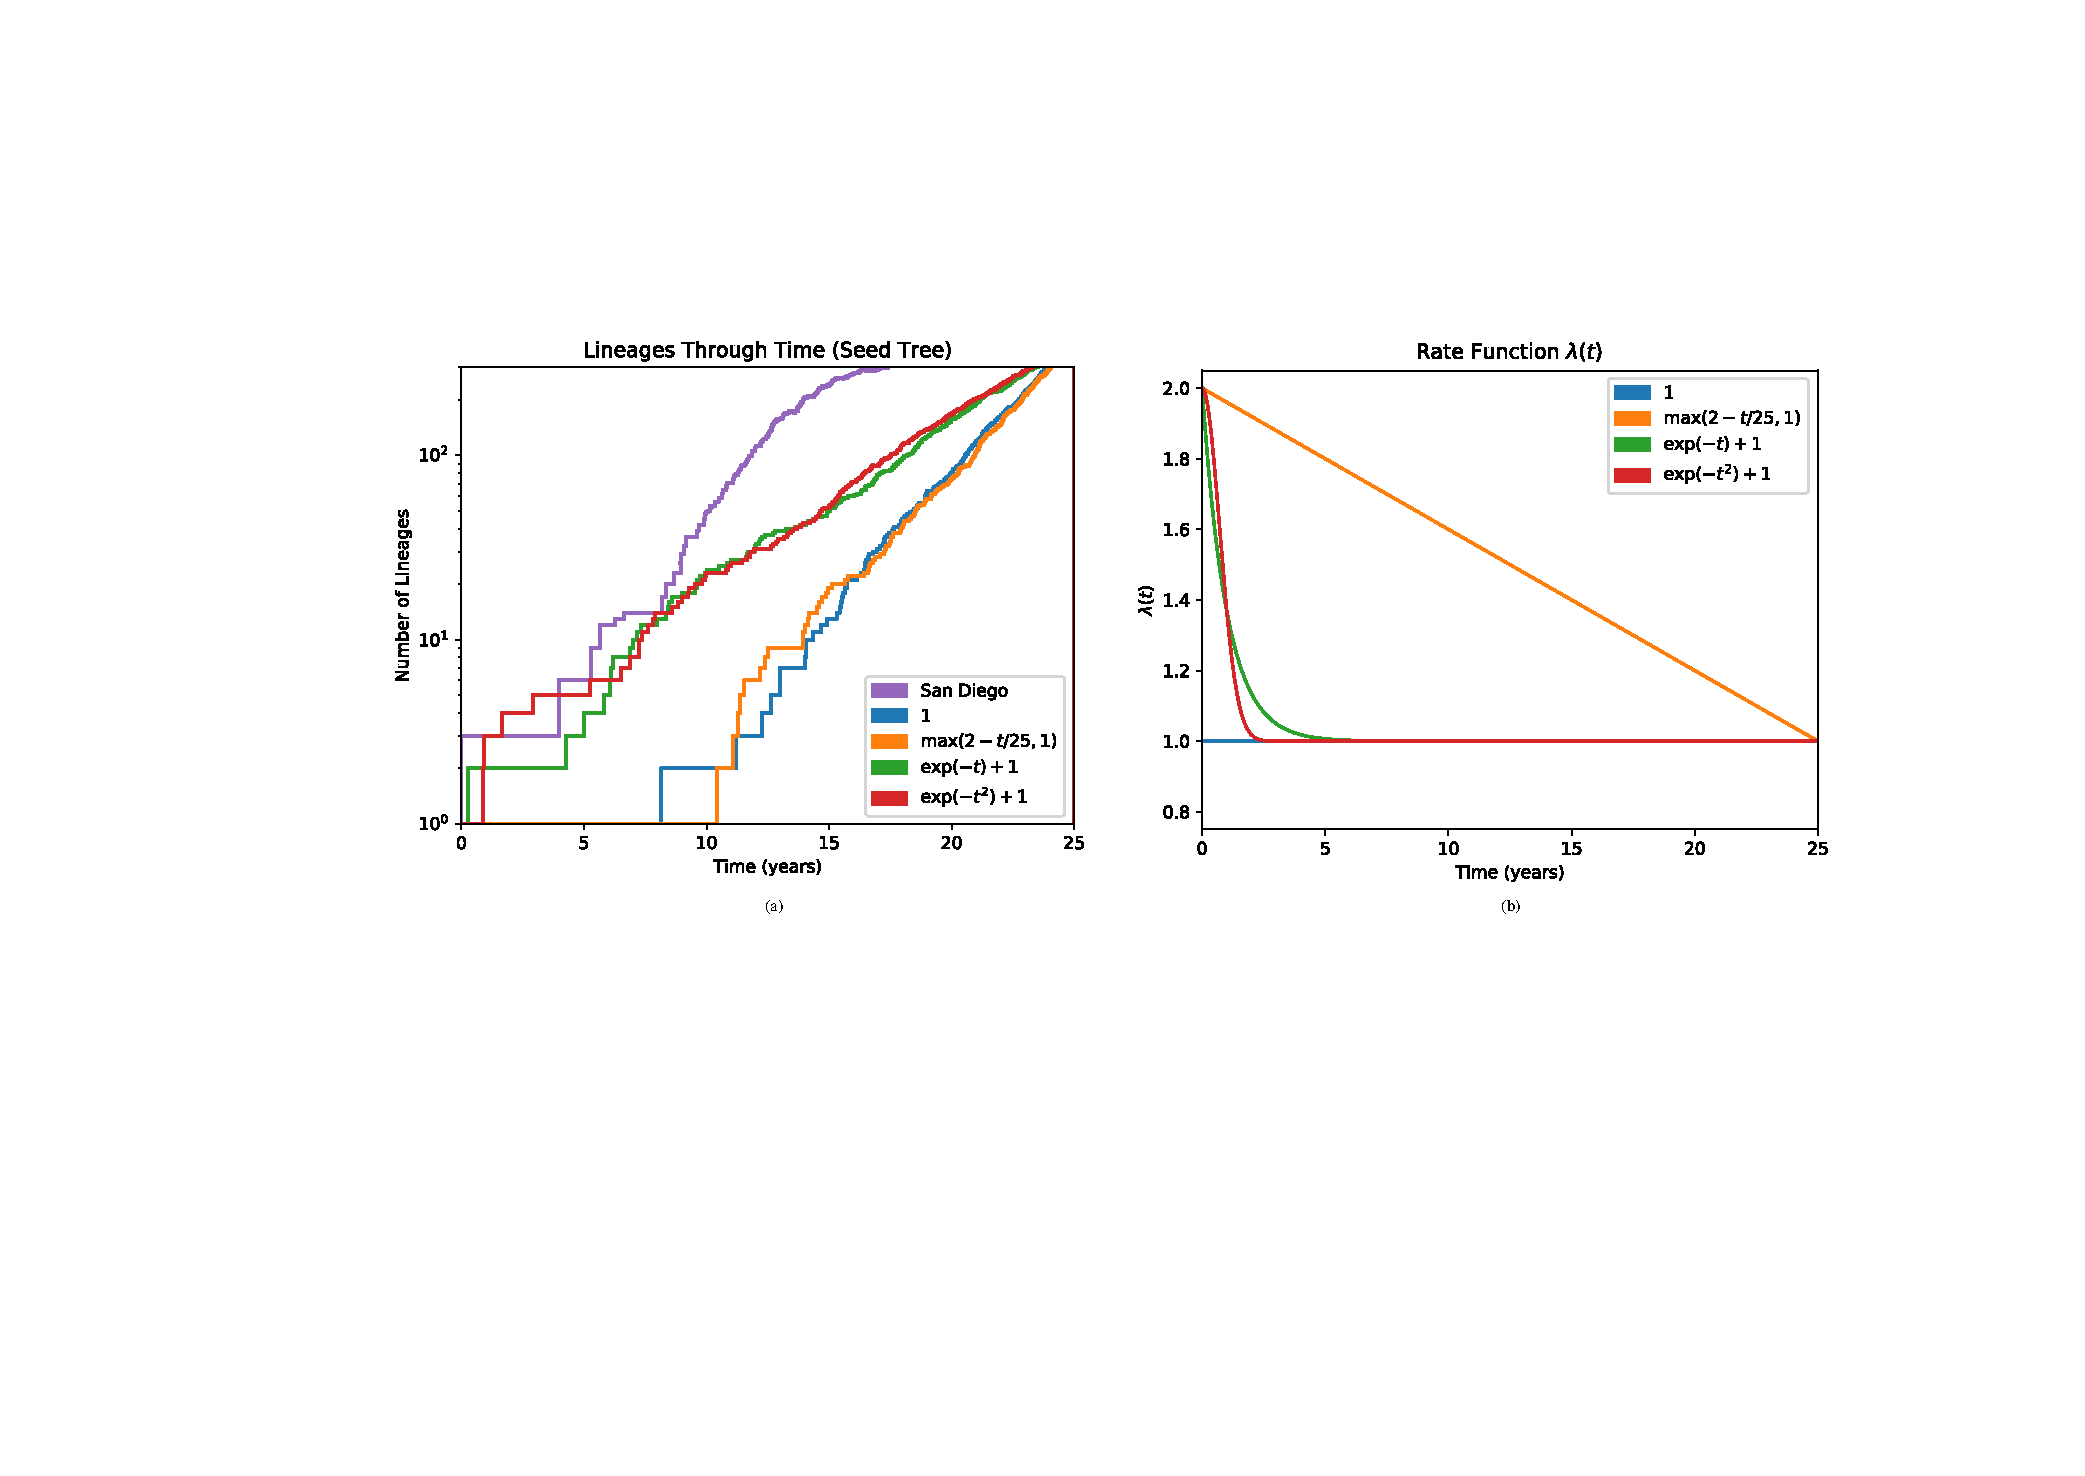
\includegraphics[width=\textwidth]{figs/favites-seed-tree}
\caption[Seed Tree]
{(a) \gls{LTT} plot of the first 25 years of the dated San Diego tree along with multiple potential rate functions for the non-homogeneous Yule model~\cite{LeGat2016}, and (b) plots of the rate functions. Because HIV trees have more short branches than normal Yule models (i.e., rate 1), we looked for functions that lead to increased numbers of lineages close to the root. This can be done by increasing the rate close to the root and then gradually decreasing the rate. As can be seen, $\lambda(t)=1$ and $\lambda(t)=\max(2-t/25,1)$ are far lower than the real San Diego curve. $\lambda(t)=\exp(-t)+1$ is much closer to the real curve, and $\lambda(t)=\exp(-t^2)+1$ is marginally closer than it. We chose to use $\lambda(t)=\exp(-t^2)+1$ as a result.}
\label{fig:favites-seed-tree}
\end{figure}

%% END FAVITES SUPPLEMENT



%% End Matter
% \printindex %% Uncomment to display the index
\bibliographystyle{ieeetr}
\bibliography{dissertation}
\singlespace

\end{document}